\newpage
\chapter{Event rate estimation}
\mbox{}\vspace{-\baselineskip}
\label{chapter_rate}

This Chapter presents an estimation of the expected event rate for the $pd\rightarrow ppn$ process that is proposed to be investigated in the $d-d$ collisions in the NICA SPD experiment in order to study color transparency (CT) effects. The estimation was performed based on the theoretical cross section approximation obtained in the framework of the generalized eikonal approach supplemented by the quantum diffusion model (QDM) of CT~\cite{Frankfurt:1996uz,PhysRevC.107.014605,Larionov:2025equ,Farrar:1988me}. A brief description of the model formalism is given in Appendix~\ref{app_formalism}. The model was adjusted to experimental data from Ref.~\cite{Cocconi:1965zz} and therefore is expected to provide realistic and reliable cross section predictions.


Figure~\ref{fig:model} presents theoretical predictions for the differential cross section of the $pd\rightarrow ppn$ process (occurring in $d-d$ collisions) as a function of the transverse momentum of the spectator neutron ($p_{st}$) for $\alpha_{s} =1$, $t=-6.8$~GeV$^2$ (which corresponds to $\theta_{\textrm{c.m.}}=49^{o}$), and $\phi=\pi$. See Chapter~\ref{Chap:kin} for the definition of the kinematic variables. 


The solid magenta curve in Fig.~\ref{fig:model} stands for the impulse approximation (IA), which corresponds to the case when only the amplitude of the hard $pp$ interaction is considered in the model, which would imply the absence of soft interactions between the final protons ($p_{3}$ and $p_{4}$) and the spectator neutron ($p_{s}$) in the initial or final state (see Fig.~\ref{fig:diagram}). This would correspond to the regime of complete (100\%) color transparency, which is however not expected to be reached at the energies of the proposed experiment. The solid blue curve corresponds to the full calculation in the framework of the generalized eikonal approximation (GEA) with all amplitudes included (both ``hard" and ``soft" parts). See Appendix~\ref{app_formalism} for more details on the model formalism.

To produce the black curves in Fig.~\ref{fig:model}, contributions from CT effects were included according to the quantum diffusion model of CT with different values of $\Delta M^{2}$, which is the model free parameter that reflects the strength of CT effects (with lower values of $\Delta M^{2}$ corresponding to stronger CT effects). As seen from Fig.~\ref{fig:model}, the dashed black curve (plotted for a low value of $\Delta M^{2}=0.7$~GeV$^2$) is close to the impulse approximation prediction, which indicates strong color transparency effects. In turn, the solid black curve (plotted for a high value of $\Delta M^{2}=3$~GeV$^2$) is closer to the full GEA calculation without CT effects, implying a relatively small CT contribution.

\newpage

\begin{figure}[htp]
\begin{center}
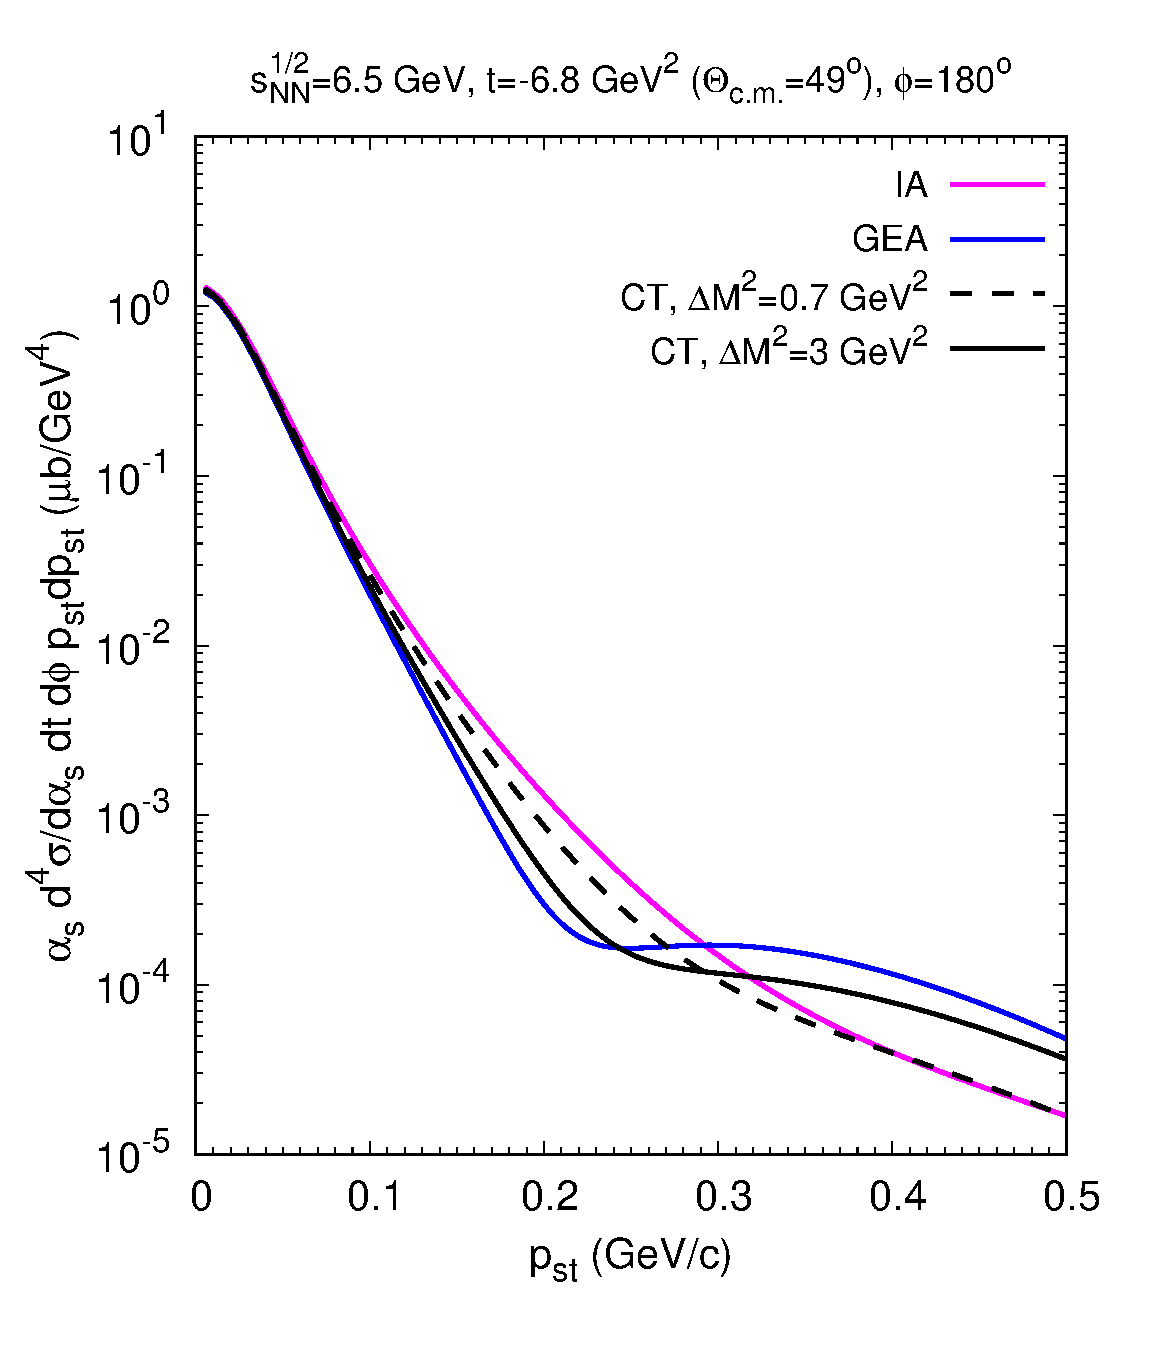
\includegraphics[width=10cm]{pictures/sig_6.5gev_35per_180deg_EventRate.eps}
\caption{\small Theoretical predictions for the differential cross section of the $pd\rightarrow ppn$ process as a function of the transverse momentum of the spectator neutron ($p_{st}$)~\cite{Frankfurt:1996uz,PhysRevC.107.014605,Larionov:2025equ,Farrar:1988me}. The solid magenta curve shows the impulse approximation (IA), while the solid blue curve corresponds to the full GEA calculation (both ``hard" and ``soft" parts). For the black curves, CT effects were included according to the quantum diffusion model of CT with different values of $\Delta M^{2}$ (specified in the plot). The calculations were performed for the following values of the remaining kinematic variables, $\alpha_{s} = 1$, $t=-6.8$~GeV$^{2}$ (which corresponds to $\theta_{\textrm{c.m.}}=49^{o}$), and $\phi=\pi$. } \label{fig:model}
\end{center}
\end{figure}



From the theoretical perspective, it would be interesting to investigate the interplay of different reaction mechanisms at different $p_{st}$ values, e.g., at lower $p_{st}\sim 0.2$~GeV/c, nuclear absorption effects are expected to dominate, while for higher $p_{st}\gtrsim 0.3$~GeV/c, rescattering of the final particles off the spectator is thought to play the major role. Therefore, experimental measurements that cover any fairly large part of the region of $0.1$~GeV/c~$<p_{st}<0.5$~GeV/c are expected to deliver new information regarding CT effects.


The strength of the CT contribution depends on the value of the momentum transferred ($Q^{2}$) and increases as $Q^{2}$ grows. This situation is illustrated in Fig.~\ref{fig:l_coh} in Appendix~\ref{app_formalism} that presents the position dependent factor $\mathcal F_{\textrm{CT}}$, through which CT effects are introduced into the reaction amplitudes in the QDM. Note that smaller values of the factor $\mathcal F_{\textrm{CT}}$ indicate larger CT effects and $\mathcal F_{\textrm{CT}} = 1$ corresponds to the absence of CT effects. As follows from Fig.~\ref{fig:l_coh}, the CT contribution is larger for higher $Q^{2}$ values. 

For a fixed value of $\sqrt{s_{34}}\simeq \frac{\sqrt{s}}{2}$, maximal CT contribution is achieved at the $Q^{2}$ values that correspond to $\theta_{\textrm{c.m.}}=90^{o}$. However, taking into account that the cross section drops quickly with $t$, measurements are proposed to be performed at $\theta_{\textrm{c.m.}}<90^{o}$, which will deliver smaller CT effects, but will allow for much higher event rate. Depending on actual experimental conditions, a compromise between the statistics and the $\theta_{\textrm{c.m.}}$ value should be found for the proposed measurements.

%\footnote[2]{Note that $Q^{2} = -t = \frac{1}{2}\left [s-4m^{2}\right ]\left [1-\textrm{cos}(\theta_{\textrm{c.m.}})\right ]$ with $m$ being the nucleon mass.}.

A dependence of the CT contribution on the value of $\sqrt{s}$ is also noteworthy. As described in Appendix~\ref{app_formalism}, higher collision energies $\sqrt{s}$ deliver larger values of the coherence length $l_{\textrm{c}}$ and consequently, a larger overall CT contribution. For this reason, measurements are proposed to be conducted at the highest $\sqrt{s}$ value accessible at the NICA collider (which is expected to be about 13~GeV). However, measurements at smaller collision energies are acceptable, too, as they will still provide a reasonable CT contribution. Also note that higher $\sqrt{s}$ values deliver lower statistics.


Furthermore, the model calculations suggest that the CT contribution changes significantly in different regions in $\phi$. Therefore (if statistics allows), we suggest to measure the $\phi$-dependence of the cross section, too. This is however not mandatory because the model analysis of the $\phi$-integrated cross section will still be capable of delivering informative conclusions about CT effects.

In addition to that, it would be preferential to restrict the value of $\alpha_{s}$ and to perform measurements at $\alpha_{s}\sim 1$ as this will select the transverse kinematics, which minimizes relativistic corrections to the deuteron wave function, and maximizes interactions in the initial and final states (ISI/FSI)\footnote[2]{The CT regime corresponds to suppressed ISI/FSI and therefore it is beneficial to perform measurements in the region of high ISI/FSI to observe the suppression effect more clearly.}.


To better understand the cross section change with $p_{st}$, Table~\ref{tab:cr_sect_est} presents cross section values for two model curves from Fig.~\ref{fig:model} (``GEA" and ``CT3") taken in four different points in $p_{st}$. In general, for a small kinematic bin $\Delta^{4}\tau = \Delta\alpha_{s} \Delta t \Delta \phi \Delta p_{st}$, the following expression can be used to estimate the number of events in this bin based on the value of the differential cross section in the center of the bin. \vspace{-0.3em}
\begin{equation}
\begin{aligned}
&\Delta N (\Delta^{4}\tau ) = \mathcal{L} \cdot \frac{\textrm{d}^{4}\sigma}{p_{\textrm{st}}\textrm{d}p_{\textrm{st}}\textrm{d}\alpha_{s}\textrm{d}t \textrm{d}\phi } \cdot p_{st} \cdot \Delta \alpha_{s} \cdot \Delta t \cdot \Delta \phi \cdot \Delta p_{st} \cdot T.\\[-8pt]
\end{aligned}\label{eq:n_events}
\end{equation}

Here $\mathcal{L}$ is the luminosity of the experiment, $\Delta \alpha_{s}$, $\Delta t$, $\Delta \phi$, and $\Delta p_{st}$ are the bin widths in all four kinematic variables, and $T$ is the duration of the experiment. In Eq.~\eqref{eq:n_events}, $\alpha_{s}$ is considered to be equal to unity, and therefore is not present in the numerator of the expression for the differential cross section.

However, for a large kinematic bin, Eq.~\eqref{eq:n_events} will not deliver precise results due to variations of the actual cross section within the bin. Therefore, to estimate event rates for the proposed color transparency measurements, the Monte Carlo simulation was performed in a large kinematic area. The event generator used for the Monte Carlo simulation employed the same theoretical model for the cross section approximation~\cite{Frankfurt:1996uz,PhysRevC.107.014605,Larionov:2025equ,Farrar:1988me}.


%\newpage

\begin{table}[htp]
\begin{center}
\caption{\small Theoretical predictions for the cross section values at four different points in $p_{st}$. ``GEA" stands for the calculations performed within the generalized eikonal approximation, while ``CT3" corresponds to the case when contributions from the color transparency effects were included in the framework of the quantum diffusion model with the free parameter $\Delta M^{2}=3$~GeV$^{2}$ (see Refs.~\cite{Frankfurt:1996uz,PhysRevC.107.014605,Larionov:2025equ,Farrar:1988me} for details). The calculations were performed for $\sqrt{s}=13$~GeV and the following values of the remaining kinematic variables, $\alpha_{s} = 1$, $t=-6.8$~GeV$^{2}$ (which corresponds to $\theta_{\textrm{c.m.}}=49^{o}$), and $\phi=\pi$.  \label{tab:cr_sect_est}}
\begin{tabular}{
   !{\vrule width 2pt}
  c!{\vrule width 1pt}   
  c!{\vrule width 1pt}
  c!{\vrule width 1pt}
  c!{\vrule width 1pt}
  c!{\vrule width 2pt}
 }
\toprule[2pt]
\multirow{2}{*}{\makecell{Model}}&  \multicolumn{4}{c!{\vrule width 2pt}}{Cross section value, $\mu$b/GeV$^4$}  \\ \hhline{|~|----|}
&  \makecell{$p_{st}=0.1~\textrm{GeV/c}$} & \makecell{$p_{st}=0.2~\textrm{GeV/c}$} &\makecell{$p_{st}=0.3~\textrm{GeV/c}$} &\makecell{$p_{st}=0.4~\textrm{GeV/c}$} \\ \hline
GEA& $20.0\cdot 10^{-3}$ & $0.30\cdot 10^{-3}$ & $0.17\cdot 10^{-3}$ & $0.12\cdot 10^{-3}$\\ \hline
CT3& $22.3\cdot 10^{-3}$ & $0.45\cdot 10^{-3}$ & $0.12\cdot 10^{-3}$ & $0.079\cdot 10^{-3}$\\  
\bottomrule[2pt] 
\end{tabular}
\end{center}
\end{table}


\begin{table}[htp]
\begin{center}
\caption{\small Estimated number of events per year for four large bins in $p_{st}$. The estimation accounts for two theoretical cross section approximations (``GEA" and ``CT3") described in the text and also in the context of Tab.~\ref{tab:cr_sect_est}. The estimation was performed based on the Monte Carlo simulation for $\sqrt{s}=13$~GeV, $\alpha_{s}=1$ and $t=-6.8$~GeV$^{2}$ (which corresponds to $\theta_{\textrm{c.m.}}=49^{o}$), using the following bin widths for the kinematic variables, $\Delta \alpha_{s} = 0.25$, $\Delta t = 2.5$~GeV$^{2}$, $\Delta \phi = 2\pi$, and $\Delta p_{st} = 0.1$~GeV/c, experiment duration $T=10^{7}$~s (1 year), and the luminosity value $\mathcal{L} = 10^{30}$~cm$^{-2}$s$^{-1}$. Numbers highlighted in red correspond to the $p_{st}=0.2~\textrm{GeV/c}$, where the largest relative difference between the two model curves is expected.  \label{tab:event_per_year}}
\begin{tabular}{
   !{\vrule width 2pt}
  c!{\vrule width 2pt}
  c!{\vrule width 1pt}
  c!{\vrule width 1pt}
  c!{\vrule width 1pt}
  c!{\vrule width 2pt}
  }
\toprule[2pt]
\multirow{2}{*}{\makecell{Model}} &\multicolumn{4}{c!{\vrule width 2pt}}{Number of events per year}  \\ \hhline{|~|----|}
 &\makecell{$p_{st}=0.1~\textrm{GeV/c}$} & \makecell{$p_{st}=0.2~\textrm{GeV/c}$} &\makecell{$p_{st}=0.3~\textrm{GeV/c}$} &\makecell{$p_{st}=0.4~\textrm{GeV/c}$} \\ \hline
GEA  &12456  &\textcolor{red}{\bf 855}  &379 &389\\\hline
CT3  &13617  &\textcolor{red}{\bf 1148}  &348 &321\\ 
\bottomrule[2pt]
\end{tabular}
\end{center}
\end{table}


\newpage



Monte Carlo events for the $pd\rightarrow ppn$ process (occurring in $d-d$ collisions) were generated at $\sqrt{s}=13$~GeV in the following kinematic area, $\alpha_{s} = 1\pm 0.125$, $t = -6.8 \pm 1.25$~GeV$^{2}$, $\Delta \phi = 2\pi$, and $p_{st}<$~0.5~GeV/c. Table~\ref{tab:event_per_year} presents the projected numbers of events per year in four large bins in $p_{st}$ estimated using the experiment duration $T=10^{7}$~s (1 year) and the luminosity value $\mathcal{L} = 10^{30}$~cm$^{-2}$s$^{-1}$. In Fig.~\ref{fig:rate_MC}, estimated numbers of events (per year) from Tab.~\ref{tab:event_per_year} are plotted as histograms, to visually illustrate the simulated event yield as a function of $p_{st}$. The blue histogram corresponds to the ``GEA" model calculation and the black histogram for the ``CT3" calculation. 



\begin{figure}[htp]
\begin{center}
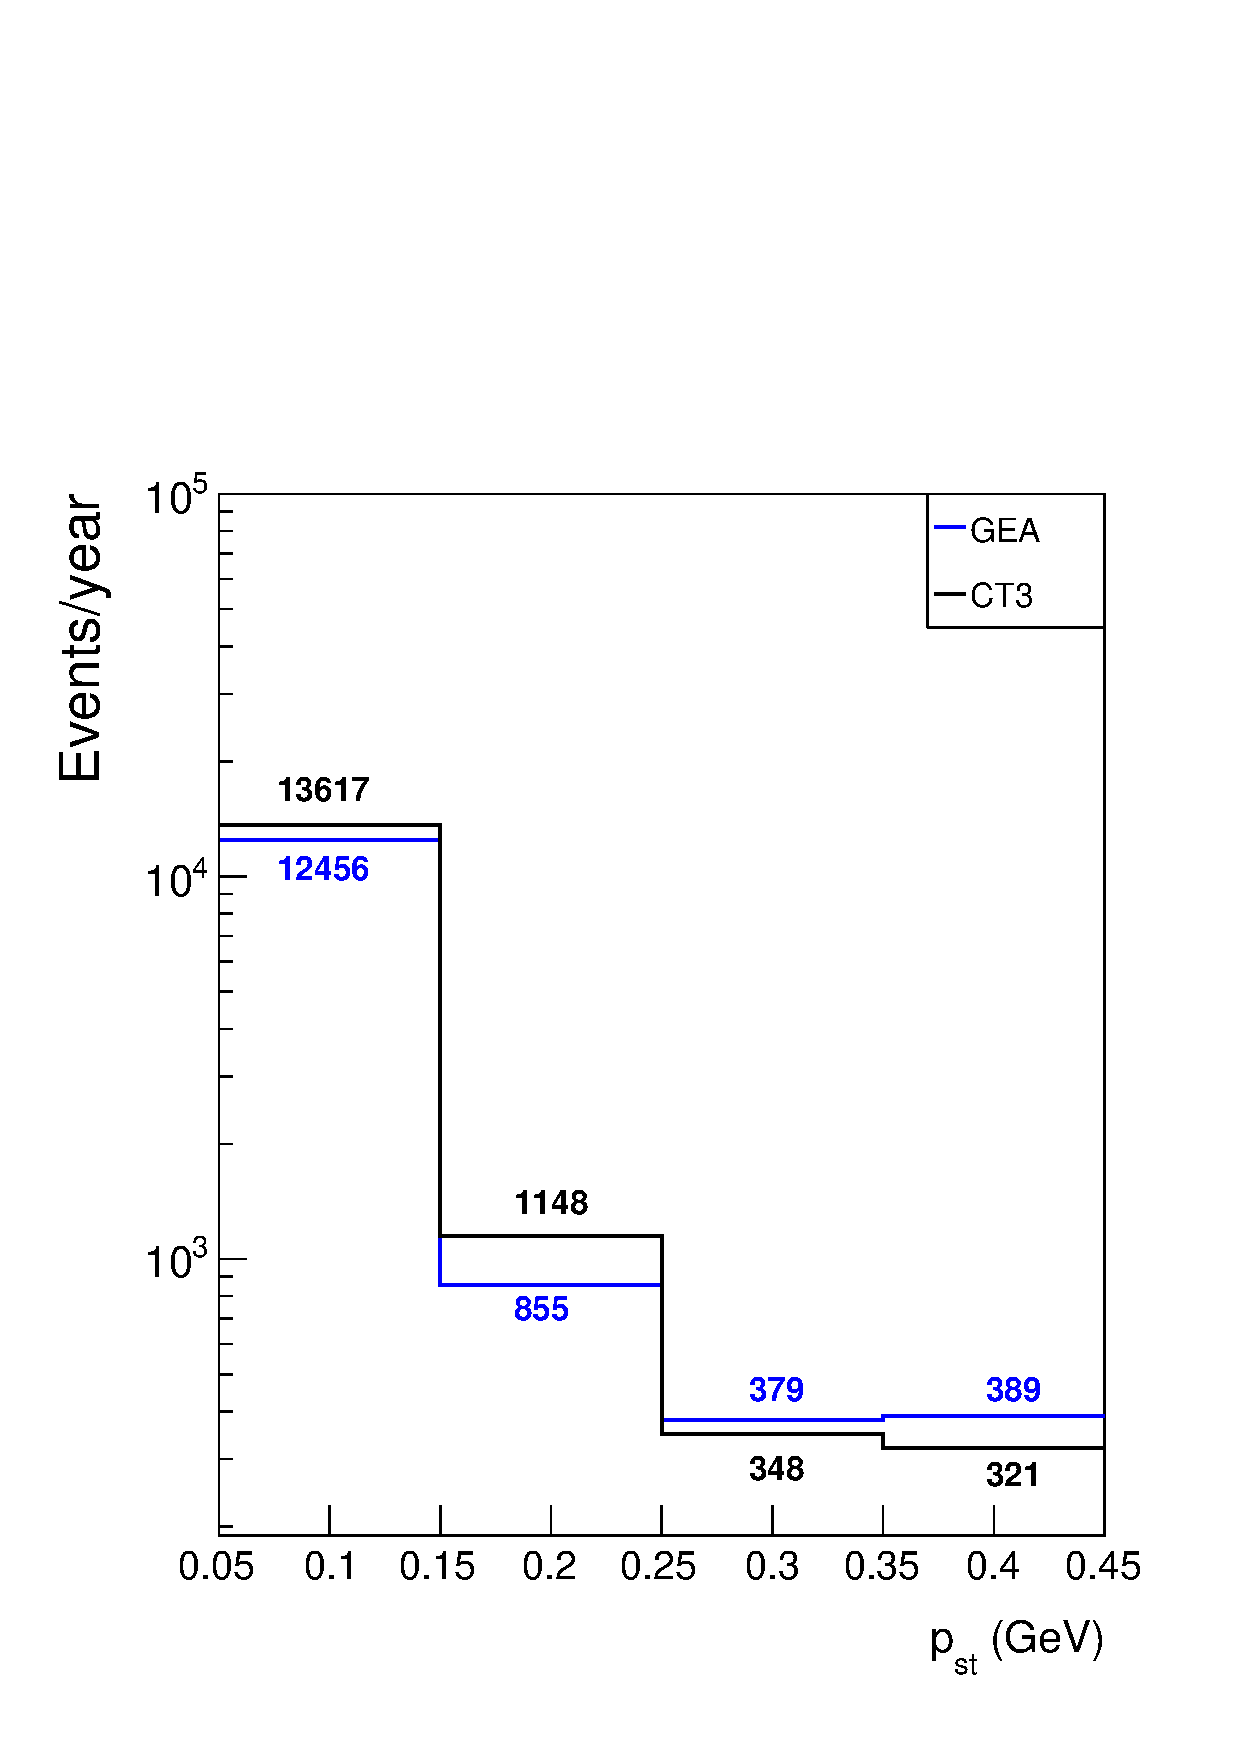
\includegraphics[width=11cm]{pictures/rate_MC_final.pdf}
\caption{\small Estimated number of events per year for four large bins in $p_{st}$. The estimation accounts for two theoretical cross section approximations: ``GEA" (blue histogram) and ``CT3" (black histogram) described in the text. The estimation was performed based on the Monte Carlo simulation for $\sqrt{s}=13$~GeV, $\alpha_{s}=1$ and $t=-6.8$~GeV$^{2}$ (which corresponds to $\theta_{\textrm{c.m.}}=49^{o}$), using the following bin widths for the kinematic variables, $\Delta \alpha_{s} = 0.25$, $\Delta t = 2.5$~GeV$^{2}$, $\Delta \phi = 2\pi$, and $\Delta p_{st} = 0.1$~GeV/c, experiment duration $T=10^{7}$~s (1 year), and the luminosity value $\mathcal{L} = 10^{30}$cm$^{-2}$s$^{-1}$. } \label{fig:rate_MC}
\end{center}
\end{figure}
\newpage


Note that in this simulation, the cuts were imposed on the $d_{1}$ momentum\footnote[3]{For the neutron $p_{s_{1}}$, both maximal transverse momentum and maximal absolute value of the longitudinal momentum in the $d_{1}$ reference frame were set to 0.1~GeV/c in the event generator.} to ensure that the neutron $p_{s_{1}}$ goes in the forward direction (see Fig.~\ref{fig:diagram} to recall the particle notations). For this reason, both histograms in Fig.~\ref{fig:rate_MC} (as well as numbers in Tab.~\ref{tab:event_per_year}) were scaled with the global factor of 0.751576 that corresponds to the integral of the wave function of the deuteron $d_{1}$ within the cuts (see more details in Ch.~\ref{Chap:kin} and also in Ref.~\cite{Larionov:2025equ}).


As seen from Tab.~\ref{tab:event_per_year} and Fig.~\ref{fig:rate_MC}, the largest statistics falls into the region of $p_{st}\sim$~0.1 GeV/c but the largest relative difference between ``GEA" and ``CT3" is observed at $p_{st}\sim$~0.2 GeV/c. Also, the region between 0.1~GeV/c and 0.2~GeV/c corresponds to a very steep statistics drop, while for higher $p_{st}$ values, change in statistics is mild. For $p_{st}\sim$~0.3~GeV/c, the relative difference between the two models is the smallest. 

From the theoretical perspective, the ``GEA" prediction corresponds to the cross section calculated within the generalized eikonal approximation without color transparency effects, while the ``CT3" prediction corresponds to the case when contributions from the color transparency effects were included in the framework of QDM with the free parameter $\Delta M^{2}=3$~GeV$^{2}$ (see Refs.~\cite{Frankfurt:1996uz,PhysRevC.107.014605,Larionov:2025equ,Farrar:1988me} for details). Therefore, for the proposed experiment, it would be helpful to estimate the statistics that would allow one to distinguish between the ``GEA" and ``CT3" cross sections on a stage of theoretical analysis in order to make a decisive conclusion regarding the CT contribution.


To perform this estimation, it is convenient to introduce the following variables, $\varepsilon$ -- the accuracy with which the absolute difference between ``GEA" and ``CT3" predictions is proposed to be measured and $f=\frac{N_{CT3} -N_{GEA}}{N_{GEA}}=\frac{\Delta N_{\sigma}}{N_{GEA}}$ -- the relative difference between the corresponding cross sections. Then the following derivations can be performed in order to estimate the desired statistics.
\begin{equation}
\begin{aligned}
\sqrt{N_{\varepsilon}} & = && \varepsilon \cdot \Delta N_{\sigma} \\
\sqrt{N_{\varepsilon}} & = && \varepsilon \cdot f \cdot  N_{\varepsilon}\\
1 & = && \varepsilon \cdot f \cdot \sqrt{N_{\varepsilon}}\\
N_{\varepsilon} &=&& \frac{1}{\varepsilon^{2} \cdot f^{2}}
\end{aligned}\label{eq:n_evt_eps} 
\end{equation}

From Tab.~\ref{tab:event_per_year}, for $p_{st} = 0.2$~GeV/c, the relative difference between the cross section values can be estimated as $f = 0.34$. Therefore, according to Eq.~\eqref{eq:n_evt_eps}, for the accuracy e.g. $\varepsilon$ = 20\%, the desired number of events $N_{\varepsilon} = 216$. Based on this estimation and also on the numbers from Tab.~\ref{tab:event_per_year} (highlighted in red), one can conclude that the projected statistics of the proposed experiment will be sufficient to reliably distinguish between the ``GEA" and ``CT3" cross section predictions (at $p_{st} = 0.2$~GeV/c, where the largest relative difference between the two model curves is expected).  


Note that in addition to statistical effects, the total cross section uncertainty is also determined by systematics. In collider experiments, a large part of the systematic uncertainty typically comes from the accuracy of the luminosity determination, and according to Ref.~\cite{Grafstrom:2015foa}, 5\%-10\% would be a reasonable estimation for the latter.

Also, taking into account a quick statistics drop in the region 0.1~GeV/c~$<p_{st}<$~0.2~GeV/c, a non-equidistant binning in $p_{st}$ might be an optimal choice for the cross section measurements. Due to a very abundant statistics around $p_{st}\sim$~0.1~GeV/c, we suggest to perform the measurements with a very small binning there (if this kinematic region is available in the experiment). In the region between 0.15~GeV/c and 0.3~GeV/c, it might be prudent to have about 3-4 bins in $p_{st}$ (depending on the statistics) to carefully scan the area of the largest relative difference between the ``GEA" and ``CT3" models, and then, fewer and larger bins for $p_{st}\gtrsim$~0.3~GeV/c.




The calculations presented in this Chapter correspond to a qualitative and conservative estimation of the event rates for the proposed experiment, which was intended to prove the overall feasibility of the proposed color transparency measurements at the energy and luminosity values that are expected to be available at NICA SPD. Based on actual experimental conditions, different variations to the suggested kinematics and/or binning should be introduced. In particular, if statistics permits, one should consider (i) more detailed binning in $p_{st}$, (ii) measuring the cross section azimuthal dependence, and possibly, (iii) measurements at higher $\theta_{\textrm{c.m.}}$. On the other hand, in case of very limited statistics, measurements should be attempted at smaller $\theta_{\textrm{c.m.}}$, where the CT contribution is smaller but the total cross section is larger as the model is still capable of making informative conclusions on CT contributions for smaller $\theta_{\textrm{c.m.}}$ (going below $Q^{2}\sim 4-5$~GeV$^{2}$ is not recommended, though).





\begin{comment}
\newpage




Theoretical predictions for the cross section values at four different points in $p_{st}$,\\ $\sqrt{s}=13$~GeV, $\alpha_{s} = 1$, $t=-6.8$~GeV$^{2}$ (which corresponds to $\theta_{\textrm{c.m.}}=49^{o}$), and $\phi=\pi$.

The estimation was performed based on the Monte Carlo simulation for $\sqrt{s}=13$~GeV, $\alpha_{s}=1$ and $t=-6.8$~GeV$^{2}$ (which corresponds to $\theta_{\textrm{c.m.}}=49^{o}$), using the following bin widths for the kinematic variables, $\Delta \alpha_{s} = 0.25$, $\Delta t = 2.5$~GeV$^{2}$, $\Delta \phi = 2\pi$, and $\Delta p_{st} = 0.1$~GeV/c, experiment duration $T=10^{7}$~s (1 year), and the luminosity value $\mathcal{L} = 10^{30}$cm$^{-2}$s$^{-1}$. 

Numbers highlighted in red correspond to the $p_{st}=0.2~\textrm{GeV/c}$, where the largest relative difference between the two model curves is expected.

$f=\frac{N_{CT3} -N_{GEA}}{N_{GEA}}=\frac{\Delta N_{\sigma}}{N_{GEA}}$
%Numbers highlighted in red correspond to the $p_{st}=0.2~\textrm{GeV/c}$, where the largest relative difference between the two model curves is expected. 


\begin{equation*}
\begin{aligned}
&F = [\mathcal{L}]\times [\mu \textrm{b}\rightarrow \textrm{cm}^{2}] \times [\Delta \alpha_{s} \Delta t \Delta \phi \Delta p_{st}] \times [\textrm{time}]\\[20pt]
&F = \left[2.7\cdot 10^{30}\textrm{cm}^{-2}\textrm{s}^{-1}\right] \times \left[10^{-30}\textrm{cm}^{2}\right] \times \left[ 0.2 \cdot 2.5 \cdot 1.047 \cdot 0.04 \right] \times \left[10^{7} s\right] = 565.38\cdot 10^{3}\\[20pt]
\end{aligned}\label{eq:rrr}
\end{equation*}

%24 \cdot 60 \cdot 60 \cdot 365~\textrm{s}

------------------------------------------------------------------------------------------

\begin{equation*}
\begin{aligned}
&p_{st}=0.2~\textrm{GeV/c}\\[20pt]
&\frac{\textrm{d}^{4}\sigma}{p_{\textrm{st}}\textrm{d}p_{\textrm{st}}\textrm{d}\alpha_{s}\textrm{d}t \textrm{d}\phi }= 1.0\cdot 10^{-3} \mu \textrm{b} /\textrm{GeV}^{4} ~~~\left[ \textrm{at}~~p_{st} = 0.2~\textrm{GeV/c},~\textrm{for}~CT3 \right]\\[20pt]
&N = \frac{\textrm{d}^{4}\sigma}{p_{\textrm{st}}\textrm{d}p_{\textrm{st}}\textrm{d}\alpha_{s}\textrm{d}t \textrm{d}\phi } \times p_{st} \times F = 1.0\cdot 10^{-3}\times 0.2 \times 565.38\cdot 10^{3} = \textcolor{red}{\bf 113}
\end{aligned}\label{eq:rrr}
\end{equation*}

------------------------------------------------------------------------------------------





\begin{equation*}
\begin{aligned}
&p_{st}=0.1~\textrm{GeV/c}\\[20pt]
&\frac{\textrm{d}^{4}\sigma}{p_{\textrm{st}}\textrm{d}p_{\textrm{st}}\textrm{d}\alpha_{s}\textrm{d}t \textrm{d}\phi }= 50.3\cdot 10^{-3} \mu \textrm{b} /\textrm{GeV}^{4} ~~~\left[ \textrm{at}~~p_{st} = 0.1~\textrm{GeV/c},~\textrm{for}~CT3 \right]\\[20pt]
&N = \frac{\textrm{d}^{4}\sigma}{p_{\textrm{st}}\textrm{d}p_{\textrm{st}}\textrm{d}\alpha_{s}\textrm{d}t \textrm{d}\phi } \times p_{st} \times F = 50.3\cdot 10^{-3}\times 0.1 \times 565.38 \cdot 10^{3} =  \textcolor{red}{\bf 2844}
\end{aligned}\label{eq:rrr}
\end{equation*}

\end{comment}

